\documentclass[border=3pt]{standalone}
% Preâmbulo compartilhado pelos diagramas TikZ da aula 14 (SLAM com EIF)
\usepackage[T1]{fontenc}
\usepackage[utf8]{inputenc}
\usepackage{lmodern}
\usepackage{amsmath}
\usepackage{xcolor}
\usepackage{tikz}
\usetikzlibrary{arrows.meta,angles,quotes,decorations.pathmorphing,decorations.pathreplacing,calc,
                positioning,shapes.geometric,shapes.misc,backgrounds,fit,
                math}

% Paleta (mesma dos SVGs originais)
\definecolor{dblue}{HTML}{2A5B8C}
\definecolor{dorange}{HTML}{B3541E}
\definecolor{dgreen}{HTML}{4A7C59}
\definecolor{dred}{HTML}{9C4B4B}
\definecolor{dcream}{HTML}{F4F1EA}
\definecolor{dshade}{HTML}{DDD7C9}

% Função gaussiana (não normalizada por padrão de escala visual)
\pgfmathdeclarefunction{gauss}{3}{%
  \pgfmathparse{1/(#3*sqrt(2*pi))*exp(-((#1-#2)^2)/(2*#3^2))}%
}

% Estilos comuns (prefixo d... para não colidir com chaves internas do pgf)
\tikzset{
  >={Stealth[length=2mm]},
  dguide/.style={gray!55, dashed, line width=0.4pt},
  daxis/.style={gray!60, line width=0.7pt, ->},
  dbody/.style={fill=black!3, draw=black!80, line width=1pt},
  dacc/.style={draw=dblue, line width=1pt},
  dlbl/.style={black!55, font=\small},
  dsub/.style={black!45, font=\footnotesize},
  dstate/.style={circle, draw=black!80, fill=dcream, line width=1pt,
                 minimum size=17mm, font=\large, inner sep=1pt},
  dobs/.style={circle, draw=black!80, fill=dshade, line width=1pt,
               minimum size=14mm, font=\large, inner sep=1pt},
  dbox/.style={rounded corners=2pt, draw=black!80, fill=dcream, line width=1pt,
               align=center, inner sep=6pt},
  dop/.style={circle, draw=black!80, fill=white, line width=1pt,
              minimum size=6mm, inner sep=0pt, font=\small},
  dtrans/.style={->, dblue, line width=1pt},
  dmeas/.style={->, dorange, line width=1pt},
  dcurve/.style={line width=1pt, dblue},
  dcurveb/.style={line width=1.4pt, dorange},
}

\begin{document}
\hyphenpenalty=10000 \exhyphenpenalty=10000 \tolerance=9999 \emergencystretch=3em
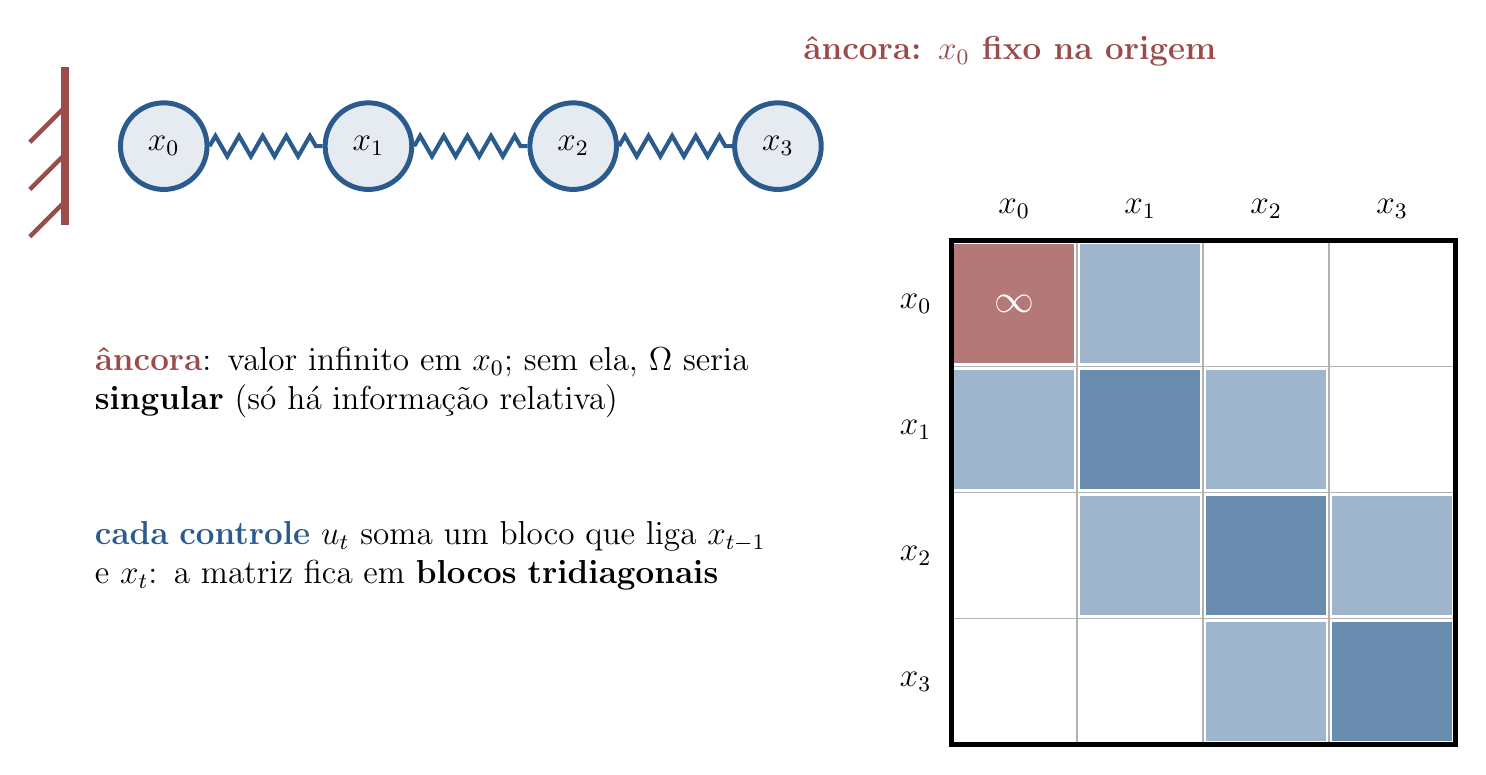
\begin{tikzpicture}[x=1cm,y=1cm]
\def\cw{1.6}
\tikzset{p/.style={circle, draw=dblue, fill=dblue!12, line width=1.8pt, minimum size=1.1cm, font=\large},
        sp/.style={decorate, decoration={zigzag, segment length=3mm, amplitude=1.3mm}, line width=1.5pt, draw=dblue}}
\foreach \i in {0,1,2,3} {\node[p] (q\i) at ({1.0+\i*2.6},6.6) {$x_\i$};}
\foreach \i/\j in {0/1,1/2,2/3} {\draw[sp] (q\i) -- (q\j);}
\draw[line width=3pt, draw=dred] (-0.25,5.6) -- (-0.25,7.6); \draw[line width=1.6pt, draw=dred] (-0.25,5.9) -- (-0.7,5.45); \draw[line width=1.6pt, draw=dred] (-0.25,6.5) -- (-0.7,6.05); \draw[line width=1.6pt, draw=dred] (-0.25,7.1) -- (-0.7,6.65);
\node[font=\large\bfseries, text=dred, anchor=west] at (9.0,7.8) {âncora: $x_0$ fixo na origem};
\foreach \i in {0,...,3} {\foreach \j in {0,...,3} {\draw[black!30, line width=0.5pt] ({11.0+\j*\cw},{3.8-\i*\cw+1.6}) rectangle ({11.0+(\j+1)*\cw},{3.8-(\i+1)*\cw+1.6});}}
\fill[dred!75] (11.04,5.36) rectangle (12.56,3.84); \node[font=\Large\bfseries, text=white] at (11.8,4.6) {$\infty$};
\foreach \i in {0,...,3} {\foreach \j in {0,...,3} {\pgfmathtruncatemacro{\d}{abs(\i-\j)} \ifnum\d=1 \fill[dblue!45] ({11.0+\j*\cw+0.04},{5.4-\i*\cw-0.04}) rectangle ({11.0+(\j+1)*\cw-0.04},{5.4-(\i+1)*\cw+0.04}); \fi}}
\foreach \i in {1,2,3} {\fill[dblue!70] ({11.0+\i*\cw+0.04},{5.4-\i*\cw-0.04}) rectangle ({11.0+(\i+1)*\cw-0.04},{5.4-(\i+1)*\cw+0.04});}
\draw[line width=1.8pt] (11.0,5.4) rectangle (17.4,-1.0);
\foreach \i in {0,...,3} {\node[font=\large] at ({11.8+\i*\cw},5.8) {$x_\i$}; \node[font=\large] at (10.55,{4.6-\i*\cw}) {$x_\i$};}
\node[font=\large, anchor=west, text width=8.6cm] at (0.0,3.6) {\textcolor{dred}{\textbf{âncora}}: valor infinito em $x_0$; sem ela, $\Omega$ seria \textbf{singular} (só há informação relativa)};
\node[font=\large, anchor=west, text width=8.6cm] at (0.0,1.4) {\textcolor{dblue}{\textbf{cada controle}} $u_t$ soma um bloco que liga $x_{t-1}$ e $x_t$: a matriz fica em \textbf{blocos tridiagonais}};
\end{tikzpicture}
\end{document}
